\documentclass[00_complete]{subfiles}

\title{Mathematical Methods}
\author{Moshe Krumbein}
\date{Fall 2021}

\begin{document}
\setcounter{chapter}{5}

\chapter{Taylor Series}
\subtitle{\theauthor~- \thedate}

\section{Introduction}

\emph{Goal:} to find an approximation for a function that is better than a
linear approximation.

\begin{symbols}[Derivatives]
    $$
    \begin{gathered}
    f',f'',f''',f^{(4)},\dots, f^{(n)} \\
    \dot f, \ddot f \text{ (derivative in terms of time)}\\
    \frac{df}{dx}, \frac{d^2f}{dx^2}, \dots, \frac{d^nf}{dx^n}
    \end{gathered}
    $$
\end{symbols}

\section{High-order derivatives of products}

$$
\begin{gathered}
    f(x)= u(x) \cdot v(x) \\
    f'=u'v+uv' \\
    \vdots \\
    f^{(3)} = u^{(3)}v+3u''v'+3u'v''+uv^{(3)}
\end{gathered}
$$

\begin{definition}[Leibniz product rule]
    \[
        (fg)^{(n)} = \sum_{k=0}^{n} \binom{n}{k}f^{(n-k)}g^{(k)}
    \]
    \begin{note}
        This is similar to \emph{Newton's generalized binomial theorem}.
    \end{note}
\end{definition}

\begin{example}
    $$
    \begin{gathered}
        f(x)=x^2\sin x \\
        f^{(n)} = \sum_{k=0}^{n} \binom{n}{k}(x^2)^{(n-k)} (\sin x)^{(k)} \\
        \text{If $n-k \geq 3$ then $(x^2)^{(n-k)}=0$. So what's left is:} \\
        f^{(n)}=
        \underbrace{\binom{n}{n}}_{1} x^2\sin^{(n)}x +
        \underbrace{\binom{n}{n-1}}_{n} 2x\sin^{(n-1)}x +
        \underbrace{\binom{n}{n-2}}_{\frac{n(n-1)}{2}} 2\sin^{(n-2)}x \\
        \boxed{f^{(n)}(x) = x^2\sin^{(n)}x + 2nx\sin^{(n-1)}x +
        n(n-1)\sin^{(n-2)}x}
    \end{gathered}
    $$
\end{example}

\section{Polynomials}

$$
\begin{aligned}
    p(x) &= a_0+a_1x+a_2x^2+ \dots + a_nx^n \\
    p'(x) &= a_1 + 2a_2x + 3a_3x^2+ \dots + na_nx^{n-1} \\
    p''(x) &= 2a_2 + \dots + n(n-1)a_nx^{n-2} \\
    p'''(x) &= 3\cdot2a_3 + \dots + n(n-1)(n-2)a_nx^{n-3} \\
    \vdots \\
    p^{(n)}(x) &= n! \cdot a_n \\
    \end{aligned} \quad
    \begin{aligned}
    p(0) &= 0! \cdot a_0 \\
    p'(0) &= 1! \cdot a_1 \\
    p''(0) &= 2! \cdot a_2 \\
    p'''(0) &= 3! \cdot a_3 \\
    \vdots \\
    p^{(n)}(0) &= n! \cdot a_n
\end{aligned}
$$

We can now rewrite $p$ in terms of its derivatives at $0$:
$$p(x) = p(0)+p'(0)x+\frac{p''(0)}{2!}x^2+\dots+\frac{p^{(n)}(0)}{n!}x^n$$
If we wanted to evaluate $p$ at a point that isn't $0$ we can do it by
utilizing transformations:

$$
\begin{gathered}
    q(x)=p(x-a) \\
    \\
    q(0)=p(a) \\
    q'(x)=p'(a) \\
    \vdots \\
    q^{(n)}(0)=p^{(n)}(a) \\
    \\
    q(x) = q(0)+q'(0)x+\frac{q''(0)}{2!}x^2+\dots+\frac{q^{(n)}(0)}{n!}x^n \\
    p(x)=p(a)+p'(a)(x-a)+\frac{p''(a)}{2!}(x-a)^2+\dots+\frac{p^{(n)}(a)}{n!}(x-a)^n \\
    \text{(Taylor series of $p(x)$ at $x=a$)}
\end{gathered}
$$

\begin{example}
$$
\begin{gathered}
    \text{Write the Taylor series of $p(x)$ at $x=-2$:} \\
    \\
    \begin{aligned}
        p(x) &= 3x^2-5x+17 \\
        p'(x) &= 6x-5 \\
        p''(x) &= 6 \\
    \end{aligned} \quad
    \begin{aligned}
        p(-2) &= 39 \\
        p'(-2) &= -17 \\
        p''(-2) &= 6 \\
    \end{aligned} \\
    \Downarrow \\
    p(x) = 39 + (-17)(x+2)+ \frac{6}{2!}(x+2)^2
\end{gathered}
$$
\end{example}

\section{Taylor Polynomial of order \texorpdfstring{$n$}{n} at
\texorpdfstring{$x=a$}{x=a} of \texorpdfstring{$f(x)$}{f(x)}}

$$
\begin{gathered}
    f(a)+ f'(a)(x-a)+ \frac{f''(a)}{2!}(x-a)^2+ \dots +
    \frac{f^{n}(a)}{n!}(x-a)^n \\
    \boxed{p^f_n = \sum_{k=0}^{n} \frac{f^{(n)}(a)}{k!}(x-a)^k}
\end{gathered}
$$
\begin{note}
    If $a=0$, then we call this polynomial a \emph{Maclaurin polynomial}
\end{note}

\section{Three Questions on Taylor Polynomials}

\begin{enumerate}
  \item For any $x$, does the taylor polynomial converge?
  \item If it does converge is it converging to the value of the function it's
      approximating?
  \item If it does converge towards the value it's trying to approximate, what
      is its \emph{error} after $n$ iterations?
\end{enumerate}

The answers to questions 1 and 2 depend on the function.

For example, the function $f(x)=e^{-\frac{1}{x^2}}$ as a Taylor polynomial is
$p^f_n=0$, which answers the first question as yes and the second as no.

If the answer of the first and second question is yes, then we can say:
$$\boxed{f(x)=\sum_{k=0}^{\infty} \frac{f^{k}(a)}{k!}(x-a)^k}$$

\begin{note}
    A \emph{series} is an infinite sum.
\end{note}

\section{What is \texorpdfstring{$n$}{n} such that we get an error which is
smaller than a specific value?}

\subsubsection{General Case}

\begin{reminder}[Lagrange's Intermediate Value Theorem]
    $$
    \begin{gathered}
        f'(c) = \frac{f(x)-f(a)}{x-a} \implies f(x)=f(a)+ f'(c)(x-a) \\
        \exists c: a < c < x
    \end{gathered}
    $$
\end{reminder}
\begin{definition}[Lagrange Remainder]
   If $f$ is continuous on $[a,x]$ (or $[x,a]$) and differential $n+1$ times
   on the aforementioned interval, then there exists a $c$ on the interval
   such that:
   $$
   \begin{gathered}
       f(x)= \sum_{k=0}^{n} \frac{f^{(k)}(a)}{k!}(x-a)^k +
       \underbrace{\frac{f^{(n+1)}(c)}{(n+1)!}(x-a)^{n+1}}_{R_n(x) -\text{Lagrange Remainder}}
   \end{gathered}
   $$
\end{definition}

\begin{example}
    Calculate $e^{0.1}$ with an accuracy of $10^{-5}$.
    $$
    \begin{gathered}
        |R_n(0.1)| < 10^{-5} \\
        R_n(0.1)=\frac{f^{(n+1)}(c)}{(n+1)!}(0.1-0)^{n+1} \\
        0 < c < 0.1 \implies e^0 < e^c < e^{0.1} \\
        R_{n}(0.1)=\frac{e^c}{(n+1)!}(0.1)^{n+1} <
        \frac{e^{0.1}}{(n+1)!}(0.1)^{n+1} < \frac{3}{(n+1)!}(0.1)^{n+1} <
        10^{-5}
    \end{gathered}
    $$
    $n=4$ definitely works, and $n=3$ does not. Therefore we can say:
    $$e^{0.1} \approx 1 + 0.1 + \frac{0.1^2}{2!} + \frac{0.1^3}{3!} +
    \frac{0.1^4}{4!}$$
    With an error that is less than $10^{-5}$.
\end{example}
\begin{example}
    Calculate $\ln1.2$ with an accuracy of $10^{-5}$.
    $$
    \begin{gathered}
        \ln(1.2) = \sum_{n=1}^{\infty}\frac{(-1)^{n+1}}{n}(0.2)^n \\
        0.2-\frac{0.2^2}{2}+\frac{0.2^3}{3}-\frac{0.2^4}{4} + \dots \\
    \end{gathered}
    $$
    \begin{definition}[Liebniz's Law]
        If we have a series with alternating signs:
        $$\sum_n (-1)^n a_n =
        \underbrace{\underbrace{\underbrace{a_1-a_2}_{S_1}+a_3}_{S_2}-a_4}_{S_3}+ \dots$$
        Where:
        \begin{enumerate}
            \item The series $a_n$ is decreasing
            \item The series $a_n$ is approaches $0$
        \end{enumerate}
        Then:
       \begin{enumerate}
            \item The sum of the entire series will always be between $S_n$ and
                $S_{n+1}$
            \item This series is called a \emph{Leibniz Series}
        \end{enumerate}

            $$\boxed{|R_n(x)| < a_{n+1}}$$
    \end{definition}
    Back to our example:

    Since our series here is a Leibniz series, then we know that:
    $$|R_n(0.2)| < \frac{0.2^{n+1}}{n+1} < 10^{-5}$$
    We can see from this that $n=7$ is a suitable answer.
\end{example}

$$
\begin{gathered}
    (1+x)^\alpha = \sum_{n=0}^{\infty} \binom{\alpha}{n}x^n
\end{gathered}
$$

\section{Leading and Sub-leading order term approximation}

Consider the Taylor Series of $f(x)$ where $x=a$:
$$
\begin{gathered}
    f(x)=f(a)+f'(a)(x-a)+\frac{f''(a)}{2!}(x-a)^2 + \dots +
    \frac{f^{(k)}(a)}{k!}(x-a)^k + \dots
\end{gathered}
$$
Let's assume that all terms before $n=k$ are zero. How will $f$ look around
$a$?

\begin{figure}[ht]
  \centering
    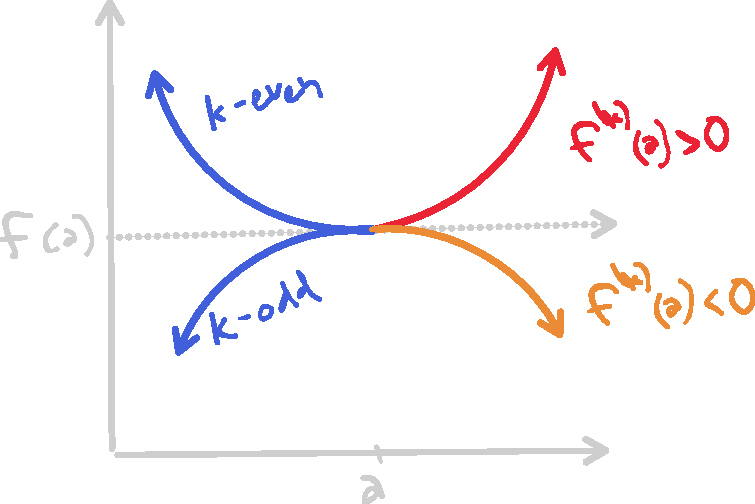
\includegraphics[width=0.5\textwidth]{w6-order}
\end{figure}

$f^{(k)}(a) > 0$ and $k$ is even: \emph{local minimum}

$f^{(k)}(a) > 0$ and $k$ is odd: \emph{inflection point}

$f^{(k)}(a) < 0$ and $k$ is even: \emph{local maximum}

$f^{(k)}(a) < 0$ and $k$ is odd: \emph{inflection point}

\paragraph{In short:}

If $f'(a) = 0$, what do we know about $a$?

We check which is the smallest $k$ (lowest derivative) such that $f^{(k)}(a)
\neq 0$.

\begin{itemize}
\item If $k$ is even then $a$ is a \emph{local extremum}.
\item If $k$ is odd then $a$ is an \emph{inflection point}.
\end{itemize}

\begin{note}
    Even if $f'(x) \neq 0$, if $f''(x)=0$, we need to check the next time
    $f^{(k)}(x) \neq 0$. If $k$ is odd, then $a$ is an \emph{inflection point}.
\end{note}

\section{Summary}
\begin{enumerate}
\item Taylor and Maclaurin polynomials
\item Maclaurin series of certain functions (and their domains)
\item Approximation of $f(x)$ until ... (Lagrange Remainder, Liebniz Series)
\item Leading and sub-leading terms (Big $O$ and little $o$ notation)
\item Investigating functions

    The line $y=ax+b$ is an \emph{asymptote} at $\infty$ if:
    $$\lim\limits_{x \to \infty} (f(x)-(ax+b)) = 0$$

    Another way of calculating $a$ and $b$ (besides for polynomial division):
    $$a=\lim\limits_{x \to \infty} \frac{f(x)}{x} \quad \quad
    b = \lim\limits_{x \to \infty} (f(x)-ax)$$
\end{enumerate}

\begin{definition}[Big $O$ notation]
    We say that $f(x)=O(g(x))$ if for some $A \in \mathbb{R}:$ $f(x) \leq
    A(g(x))$.
    $$f(x)=\frac{1}{2}x^2+2x-1 = O(x^2) \quad x \to \infty$$
    We say that $O(x^2)$ the "most dominant term" or the "size" of the function
    $f(x)$.

    As far as we're concerned, if the leading term of a Taylor series is
    $\frac{f^{(k)}(a)}{k!}(x-a)^k$, we say that around the point $a$:
    $$f \approx O((x-a)^k)$$
    and that $f$ zeros at $a$ of the $k$-th order.
\end{definition}
\begin{definition}[little $o$ notation]
        $$f \approx o(g(x)) \quad f \ll g(x)$$
\end{definition}
\begin{example}[Big $O$ and little $o$ notation]
    $$x^6+1 = O(x^6) \quad \quad x^6+1 = o(x^7)$$
\end{example}
\begin{definition}[L'H\^{o}pital's rule]

    L'H\^{o}pital's rule helps us calculate limits of the form: "$\frac{0}{0}$"
    or "$\frac{\infty}{\infty}$".
    $$\lim \frac{f(x)}{g(x)} = \lim \frac{f'(x)}{g'(x)}$$
    \begin{example}
        $$
        \begin{gathered}
            \lim\limits_{x \to 0} \frac{1-\cos 10x}{x^2} \overset{L'H}{=}
            \lim\limits_{x \to 0} \frac{10\sin 10x}{2x}  \overset{L'H}{=}
            \lim\limits_{x \to 0} \frac{100\cos 10x}{2} = 50
        \end{gathered}
        $$
    \end{example}
\end{definition}

\begin{definition}[Weierstrass extreme value theorem]
    If $f$ is continuous on $[a,b]$, then $f$ has a \emph{minimum} and
    \emph{maximum} on $[a,b]$.
\end{definition}

\begin{example}[function as a Taylor Polynomial]
    $$
    \begin{gathered}
        \ln(1-5x^2) \\
        \\
        \ln(1+x) = \sum_{n=1}^{\infty} (-1)^{n+1} \frac{x^n}{n} \\
        \ln(1-5x^2) = \sum_{n=1}^{\infty} (-1)^{n+1} \frac{(-5x^2)^n}{n} =
        \sum_{n=1}^{\infty}- \frac{5^n}{n}x^{2n} \\
        \\
        -1 < -5x^2 \leq 1 \implies -\frac{1}{5} \geq x^2 > \frac{1}{5} \implies
        -\sqrt{\frac{1}{5}} < x < \sqrt{\frac{1}{5}}
    \end{gathered}
    $$
\end{example}
\end{document}
